\documentclass[11pt]{article}
\usepackage{mgates-letter}
\definecolor{dark_blue} {rgb}{0., 0., 0.65}
\usepackage{makecell}
\usepackage{listings}
\usepackage{textcomp}
\usepackage{mathrsfs}  % mathscr font
\usepackage{boxedminipage}
\usepackage{rotating}
\usepackage{csquotes}
%\usepackage{natbib}
\usepackage[colorlinks, filecolor=dark_blue, urlcolor=dark_blue, linkcolor=black, citecolor=black]{hyperref}

\usepackage{cleveref}
\begin{document}
\sloppy
\begin{center}
	{{
		\Large{
			\textsc{PhD Programme in Computer Science and Engineering \\ 
			\vspace{4mm}
			Cycle XXXVI}
			}
	}} 
	\rule[0.1cm]{\textwidth}{0.1mm}
	\rule[0.4cm]{\textwidth}{0.6mm}
\end{center}

\begin{center}
	{\LARGE{Engineering Cyber-Physical Swarms with Aggregate Computing}} \\
	\vspace{4mm}
	{\large{PhD Thesis proposal}} 
	\vspace{4mm}
\end{center}
\vspace{8mm}
\par
\noindent
\begin{minipage}[t]{0.47\textwidth}

{\large{Commission: \\\bf
Prof. Mirko Viroli \\
Prof. Andrea Omicini \\
Prof. Matteo Ferrara} 
}
\end{minipage}
\hfill
\begin{minipage}[t]{0.47\textwidth}
	\raggedleft
	{
		\large{PhD Student: \\\bf Gianluca Aguzzi}
	}
\end{minipage}
\vspace{10mm}

{
	\raggedright
	\rule[0.1cm]{\textwidth}{0.6mm}
	\rule[0.5cm]{\textwidth}{0.1mm}
}

\newcommand{\scafiweb}{{ScaFi-Web}}
\newcommand{\acfull}{{aggregate computing}}
\newcommand{\ac}{{AC}}
\newcommand{\marl}{{MARL}}
\newcommand{\rl}{{RL}}
\newcommand{\scafi}{{ScaFi}}
\newcommand{\cpsw}{{CPSw}}
\newcommand{\rev}[1]{{
	%\color{red}
	#1
	}}
\abstract{
	This thesis aims to define a path towards the engineering of ``Cyber-Physical Swarms" (\cpsw{}) - where artificial swarms are seen in a modern key, including swarm robotics, large-scale IoT scenarios, and crowd engineering (tracking and control). 
	%
	\cpsw{} are backed by emerging trends of autonomic, pervasive, ubiquitous computing that foster a vision of distributed systems composed of a considerable number of simple entities that collectively perform collective tasks.
	%
	These systems are similar to natural social-animal groups, where plentiful animals (like ants, sheep, \dots) achieve shared population-wide goals.
	%
	Furthermore, these behaviour are typically achieved through self-organisation, making the system robust to failures and highly scalable.
	%
	Inspired by nature, we define the notion of ``Cyber-Physical Swarms'' -- the extension of `swarms' in computer science.
	%
	Engineering this kind of system with traditional approaches is inadequate, 
	due to the distributed control, high-rate failure, openness, and local-to-global behaviour mapping.
	%
	Therefore, my thesis is focused on finding a systematic and reproducible way to design \cpsw{}. 
	In particular, we plan to leverage \acfull{} -- a novel top-down global-to-local programming model.
	%
	As a final result of my PhD, we intend to analyse the application of \acfull{} in \cpsw{}. This will touch on several aspects like distributed intelligence, flexible and opportunistic middlewares, building blocks and ad-hoc API.
}
\newpage
%\tableofcontents
\section{Introduction}
The recent evolution of IT technologies fosters a vision in which computation is \textit{everywhere}. Several modern paradigms advance that vision, like ubiquitous~\cite{DBLP:journals/sigmobile/Weiser99}, pervasive~\cite{DBLP:journals/computer/SahaM03}, collective~\cite{DBLP:journals/computer/Abowd16}, and automatic computing~\cite{DBLP:journals/computer/KephartC03}.
%
These consider systems (typically \emph{cyber physical}) where a large number (hundreds - thousands - millions) of simple interacting devices collectively perform complicated tasks in a decentralised manner, acting and sensing through a shared environment. 
%
Thus, they can be conceived as \textit{complex} systems like the ones observed in nature.
%--  by means that we cannot understand the behaviour of the whole looking only at the parts.
%
Speaking about \textit{natural} complex systems, social animals, like a swarm of insects, exhibit fault-tolerant, effective, and efficient collective behaviours leveraging self-organisation.

Consequently, we want to promote cyber-physical systems with the properties observed in swarms, thus we came to define \textit{Cyber-Physical-Swarms} (\cpsw{}): a collection of (simple) computational entities linked with the physical world via perception and actuation that reach collective goals through self-organising behaviours.
%
Swarm robotics, ``swarms” of people (crowds) or, in general, ``swarms” of IoT devices are clearly defined instances of \cpsw{}.

Traditional design (device-level) methodologies are inadequate for \cpsw{} engineering, due to local-to-global mapping problems, distributed control, complex IT infrastructures and scalability concerns.
%
To overcome these issues, the goal of my research PhD thesis is to find a systematic methodology (models, techniques and algorithms) to synthesise and deploy self-organising behaviours with predictable outcomes for \cpsw{}.

This is not the first effort that wants to tackle these kinds of problems. Traditionally, designers have been guided by natural phenomena observation that was then transposed into computer systems -- a so-called
bottom-up approach. However, this methodology led to specific solutions that hardly scale up with application complexity thanks to composability.
%
Novel techniques -- and the one that we follow in this work -- consist of top-down global-to-local approaches where designers define the system outcome directly at the collective level.
%
Among the many (like Buzz~\cite{DBLP:journals/software/PinciroliB16}, TOTA~\cite{DBLP:conf/icdcsw/MameiZL03}) in this thesis, we will take into consideration \textit{\acfull{}} (\ac{})~\cite{DBLP:journals/computer/BealPV15} since it enables the definition of self-organising collective behaviours that can be composed functionally. In this way, the \textit{aggregate} programs (i.e. programs written using \ac{}) can be reused in different domains and can scale with domain complexity. 

Even if \ac{} is applied already in different scenarios like crowds of people~\cite{DBLP:journals/computer/BealPV15}, smart cities~\cite{DBLP:journals/isci/CasadeiFPRSV19}, and large-scale IoT~\cite{DBLP:journals/fgcs/CasadeiFPRSV19}, it currently lacks software architectures (middleware), systematic program definition, abstraction layers (API) and foundational aspects.
%
Consequently, my thesis aims to investigate and analyse critically \acfull{} techniques in the field of \cpsw{}.
%
This investigation will address multiple directions like distributed intelligence, flexible middlewares, and ad-hoc building blocks, possibly leading to contributions both at a foundational (i.e. building blocks, \ac{} language, API) and ``architectural" level (middleware, message passing architecture, ...).
%
In this process, Machine Learning (ML) -- and in particular Reinforcement Learning (\rl{}) -- techniques will be used in support of \acfull{}~\cite{research} to improve adaptivity, efficiency and efficacy

The proposal is then structured as follow. In \Cref{background} I discuss the current state-of-the-art methodologies and related works in the field \cpsw{} behaviour definition.
%
In \Cref{contribution} I devise my thesis contribution in the path of engineering predictable outcome in \cpsw{}. In this section, I also show the preliminary works done in this first PhD year
%
Finally, in \Cref{future} I describe what are the activities that I plan to do in the rest of my PhD project.

\section{Background} \label{background}
The goal of this section is to clarify what we mean with \textit{Cyber-Physical Swarms}, what systems are similar to our definition, and what research areas have to deal with similar problems.
\subsection{Cyber-Physical Swarms}
This term is used to describe many computational nodes that collaborate to solve collective problems similar to what we observe in natural ``swarm'' systems.
%
These systems have a large population of networked nodes (hundreds -- thousands), and they are typically \textit{open} (i.e. we cannot know the total node number apriori). Consequently, the collective behaviour should be \textit{scale-independent} (i.e. the same program must work in small networks as well as in very large networks).
%
Besides, nodes are associated with a \textit{physical} asset through sensors and could change the environment using actuators. Namely, they have an embodiment in the world -- so the name of cyber-physical. 

The nodes could be heterogeneous, but we imagine a \emph{homogenous} local behaviour (i.e. each node should execute the same local logic). Furthermore, nodes act collaboratively, and are not selfish -- they always operate for the global collective utility.

We suppose that the overall system could not use a central entity -- so we need to deal with distributed control. Even if modern architectures could be used (e.g cloud/edge infrastructures), in general, we need to react to local problems quickly. Hence, moving this decision far from the physical assets could be dangerous (since they are a kind of \emph{critical systems}).
%
As a concluding note, we are interested in the \textit{macro-level} behaviour and not at the \textit{micro-level}. Hence, we intend to describe the collective not by emergence, but by defining a global wanted structure.

\cpsw{} is a kind of Complex Adaptive system~\cite{holland1992complex}, but our vision enforces properties that are not necessarily present in standard complex systems' definition, like the large agents' number and the collaborative agents' nature.
%%
Collective Adaptive Systems~\cite{DBLP:journals/corr/abs-1108-5643} is near to our \cpsw{} description but in our definition agents pursue \emph{collective} (not individual) goals, and they have a homogenous behaviour.
\subsection{Swarm Intellingece}
Swarm intelligence has a similar starting point to our approach since it tries to use the tactics observed in social animals in swarm robotics. The behaviours are derived in a bottom-up fashion, hence designers have tried to achieve a collective behaviour through emergence observing local animal behaviours.
%
For instance, artificial stigmergy~\cite{DBLP:journals/fgcs/DorigoBT00} derives from that studies. But, nowadays, swarm intelligence is more focused on algorithms. 
Indeed, the collective behaviours observed in nature are leveraged to perform \textit{optimisation} strategies or to directly solve problems by searching in the solution space.
%%
There are several examples of swarm intelligence optimisation algorithms, such as Ant Colony Optimisation (ACO)~\cite{DBLP:journals/tsmc/DorigoMC96}, Particle Swarm Optimisation (PSO)~\cite{DBLP:conf/icnn/KennedyE95} and Flock of Starling Optimisation (FSO)~\cite{DBLP:series/sci/FulgineiS11}.

Even if they are important approaches, we are not directly interested in them. Indeed, we take \textit{inspiration} from swarms but only to achieve similar behaviour in the artificial swarm leveraging self-organisation. We do not want to \textit{mimic} nature but leverage the same mechanism to reach robust collective systems.
\subsection{Swarm Robotics}
Historically, swarm robotics started from the first Swarm intelligence approaches. Then, it has emerged as the \textit{engineering} part of that branch. Indeed, the general goal of \emph{swarm engineering} is \emph{to define systematic and well-founded procedures for modelling, designing, realising, verifying, validating, operating, and maintaining a swarm robotics system}~\cite{DBLP:journals/swarm/BrambillaFBD13}.

In Swarm Robotics, the focus is mainly on \textit{robots} that are \emph{autonomous}, \emph{situated}, and with \emph{no central control}. We aim to expand this vision also to other ``swarm-like'' systems, such as a crowd of people, large scale IoT and smart cities where we do not have robots. 

In particular, the novel branch of \textit{automatic design}~\cite{DBLP:journals/firai/FrancescaB16} is very appealing to be used in \cpsw{}. In autonomic design approaches, the controller is derived through \textit{genetic algorithms} or \textit{Multi-agent Reinforcement Learning} following a \textit{global} utility function. 
\subsection{Multi-Agent Systems}
A \cpsw{} could be seen as a multi-agent system and in particular a \emph{many}-agent system where a group of autonomous entities are programmed to achieve collective behaviours through \emph{repeated} sensing, computation, communication, and actuation.

Due to the high stochasticity of the environment, it is almost impossible to know and program the optimal behaviour for all agents in advance.

This uncertainty results in creating intelligent agents so that they can \emph{learn} the optimal behaviour and adapt to environmental changes.
\subsubsection{Learning}
In recent decades, there has been an emerging trend in the use of \rl{} 
in multi-agent settings -- called Multi-Agent Reinforcement Learning (\marl{}) -- as a powerful, robust and adaptive learning paradigm.
%
Progress has been considerable, and a broad of algorithms are now available.

\marl{} is a conjunction of Game theory and \rl{}, 
 and there are several (even orthogonal) viewpoints on which researchers have been focused.
First attempts from \rl{} viewpoint, 
 goes towards a so-called \textit{independent learning}~\cite{DBLP:journals/tsmc/BusoniuBS08} approach, where each agent learn locally against the whole environment~\cite{DBLP:conf/icml/Tan93}.

%%% Put reference to independent learning overview
The pro of these approaches is that they can scale up with the number of agents, 
 but, unfortunately, the learning process is extremely non-stationary and unstable.
% 
%Furthermore, they are heuristic and do not exist any convergence proof (even if, in practice, they often reach a good policy).

Other efforts have focused on achieving game-theoretic properties, such as Nash-equilibrium of Pareto optimality.
The problem is that it is used with few agents and scale hardly with the application complexity.
%
Finally, current emerging trends tend to leverage a so-called centralised training and decentralised execution (CTDE)~\cite{DBLP:journals/tcyb/NguyenNN20} approach, by which 
 agents should leverage the system-wide knowledge at training time and then at runtime they act independently~\cite{DBLP:journals/aamas/Hernandez-LealK19}. In this setting, Deep Learning is typically employed, reaching and exceeding the state-of-the-art traditional \marl{} algorithms.
 
The main problem with most of the solutions available in the literature is that they consider a small number of agents (or at least test them on small games) --- even if some novel trends exist, like Mean Field Reinforcement Learning~\cite{DBLP:journals/corr/abs-2108-02731}.
Furthermore, in \cpsw{} we are mainly interested in learning algorithms that tackle homogenous behaviour, i.e. the policy founded could be shared with the entire collective. This will ease training phases of numerous agents, reducing the non-stationary and state-action space

This section cannot be exhaustive, \marl{} is a newly emerging research direction and multiple different viewpoints exist. The articles \cite{DBLP:journals/aamas/Hernandez-LealK19, DBLP:journals/corr/abs-1911-10635, DBLP:journals/corr/abs-1908-03963} give a comprehensive overview of current state-of-the-art solutions and ideas.
\subsection{Aggregate Computing}

\ac{} is an approach to specify \emph{self-organising} behaviours from a global perspective.
%
The aggregate program (i.e. a program written with \ac{}) provides a way to map the local observations of an individual agent (i.e., sensing information, current agent state, and inbound messages from neighbours) to (eventually) globally-coherent local actions
 (i.e., actuation instructions and outbound messages).
%

Historically, aggregate programming originated from works drawing inspiration from nature: whereas the biological inspiration led to swarm intelligent MASs, where agents indirectly interact by pheromones \cite{DBLP:conf/atal/ParunakBS02}, the physical inspiration led to the idea of agents acting in environments empowered with potential fields \cite{DBLP:journals/trob/HwangA92}.
%
Recently, aggregate programming has been formally backed by \emph{field calculi}~\cite{viroli2019jlamp-si-coord}, which provide a compositional approach
 to global behaviour specification
 based on functions from fields to fields.
%
A \emph{(computational) field} is a map associating a value to any device of a given domain.
%
So, for instance, controlling the movement of a swarm of drones can be expressed through a field of velocity vectors, which maps any drone of the swarm to a corresponding velocity (speed and direction); the set of low-energy devices can be denoted through a Boolean field holding \texttt{true} for devices whose local energy level (as perceived by local sensors, and collectively also denoted as a floating-point field) is under a certain threshold (also a floating-point field).
%
These fields, then, are generally manipulated through three kinds of constructs:
\begin{enumerate}
\item \emph{stateful evolution}: \lstinline|rep(init)(f)|---expressing how a field, starting as \lstinline|init|, should evolve round-by-round through unary function \lstinline|f|.
\item \emph{neighbour interaction}: \lstinline|nbr(e)|---used to exchange with neighbours the value obtained by evaluating field expression \lstinline|e|; this locally yields a \emph{neighbouring field}, i.e., a field that maps any neighbour to the corresponding evaluation of \lstinline|e|.
\item \emph{domain partitioning}: \lstinline|branch(c){ifTrue}{ifFalse}|---used to partition the domain of devices into two parts: the devices for which field \lstinline|c| is locally \lstinline|true|, which evaluate expression \lstinline|ifTrue|, and those for which \lstinline|c| yields \lstinline|false|, which evaluate \lstinline|ifFalse|. 
\end{enumerate}

The idea of aggregate programming is to write programs talking about global behaviour (fields) and let these drive the local activity of every device in the system.
%
An aggregate program needs to continuously compute and communicate with neighbours to yield a collective adaptive behaviour.
%
An individual atomic step involving context acquisition, computation of the program, and neighbourhood-based communication is called \emph{round}.
%
In detail, a \emph{round} that runs at some device consists of:
\begin{enumerate}
  \item \emph{context acquisition}: the device collects information from the sensors, the messages from neighbours (including the device itself---to model state);
  \item \emph{program evaluation}: the aggregate program is evaluated against the acquired context, yielding an export, namely the message to be sent to neighbours;
  \item \emph{export sharing}: the export is sent to the neighbours;
  \item \emph{actuations}: the export also includes information that can be used to drive actuators in the local node.
\end{enumerate}

Rounds execution is completely asynchronous, so there is no global clock or barrier to coordinate the aggregate. This makes it possible to scale easily with the number of nodes. 
%
The combination of the logic of the aggregate program and such a collective, proactive, and periodical execution can promote the pursuit of collective adaptive behaviour

\ac{} is embodied by concrete aggregate programming languages~\cite{viroli2019jlamp-si-coord},
 such as \scafi{}~\cite{DBLP:conf/isola/CasadeiVAD20,DBLP:journals/eaai/CasadeiVAPD21},
 a Domain-Specific Language (DSL) embedded in Scala
 as well as a toolchain for aggregate system development and simulation~\cite{Casadei2016mass}.
%

As target toolkit, we will adopt \scafi{} in this my thesis work mostly for practical reasons: concerning other aggregate programming languages such as Proto and Protelis, surveyed in \cite{viroli2019jlamp-si-coord},
\scafi{} is a \emph{strongly typed}, \emph{internal} DSL; therefore, it enables straightforward reuse of powerful features from the Scala host language (including its type system, type inference, programming abstractions, libraries).

Additionally, ScaFi also represents an agile framework for testing experimental language features (cf. \emph{aggregate processes}~\cite{DBLP:journals/eaai/CasadeiVAPD21}.
%
Hence, among the existing languages for aggregate programming, we believe \scafi{} is the one better fitting rich scenarios like what we expected for \cpsw{}.
%
Finally, we typically leverage simulations to verify collective behaviours specifications since it is costly to set up a large scale bench test. In this context, Alchemist~\cite{} is the standard de-facto to simulate aggregate programs, and this will be our reference for verifying our results~\cite{Pianini_2013}.

A full account of research about aggregate programming, field calculi, and \scafi{} is beyond the scope of this proposal; more details can be found in~\cite{viroli2019jlamp-si-coord,DBLP:journals/eaai/CasadeiVAPD21}.

\section{Contribution} \label{contribution}
\subsection{Thesis proposal}
\begin{figure}
	\centering
	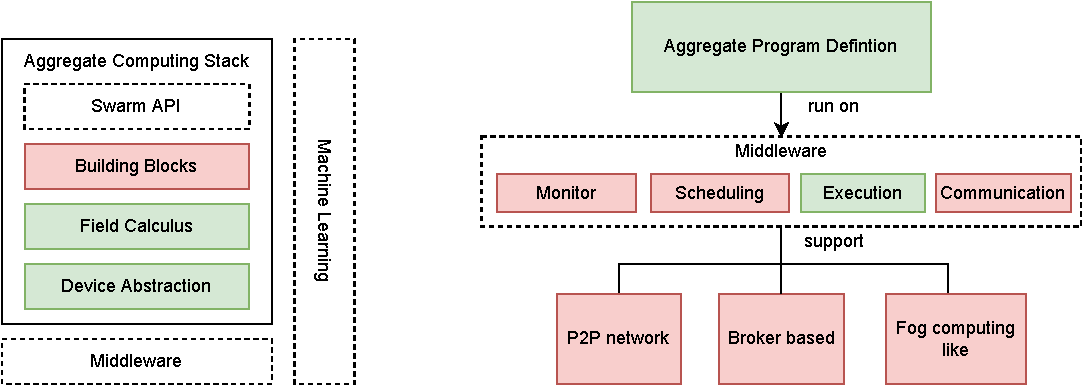
\includegraphics[width=\textwidth]{img/to-do-for-thesis.pdf}
	\caption{Devises the current status of \ac{} toolkit in literature. Dotted blocks mean a lack of that concept. Green blocks are the ones that can be considered stable and reusable in \cpsw{} engineering. Red blocks are the ones that currently exist but need to be expanded in order to support \cpsw{}.}
	\label{fig:current-state}
\end{figure}
My PhD thesis will be focused on the engineering process of \cpsw{} leveraging \ac{} abstractions. The choice of \ac{} as a conceptual model for describing \cpsw{} behaviours is well fitted since it:
\begin{itemize}
	\item allows defining collective behaviours robust (against failure, environmental perturbations, \dots{}) and scale-independent: the aggregate programs are expressed through manipulation of computational field, abstracting over nodes itself and treating the systems like a computational blob that evolves in time. In doing that, the logic is independent of the node population, so it natively handles failure and openness, and the same program can be applied to very dense IT networks;
	\item enhances the possibility to \textit{program} self-organisation: Typically, self-organisation is something that was achieved by observing natural phenomena. \ac{} provides a systematic way to let \textit{self-organising} behaviour programmable. To do that, the programs are defined using a composition of building blocks that expose self-organising patterns;
	\item is applicable to different deployment kinds leveraging modern complex IT infrastructures: Aggregate program does not depend on any particular IT network framework. Potentially, it could be applied in cloud-like systems, P2P networks and client and server architecture. This is particularly important for \cpsw{} since they could be deployed in different kinds of networks.
\end{itemize}

This choice impact strongly on the design process of collective application.
%
Currently, however, there is still a gap between the application of \ac{} and its use in CPSw. 
%
In fact, great strides have been made in research from a foundational point of view, but an all-encompassing approach to the design and implementation of collective programmes is still lacking, and this is where my thesis will be focused on.
%
In particular, my works will be focused at:
\begin{itemize}
	\item developing a \textit{flexible} middleware: 
	developing middleware for \ac{} must consider several aspects such as message delivery, distributed monitoring, neighbour discovery, deployment techniques and round frequency. Not much work has been done in this direction yet. One of the most important ones is \emph{pulverised architecture}\cite{DBLP:journals/fi/CasadeiPPVW20} that wants to make aggregate programs applicable to various deployment kinds. Hence, we would expand that \emph{pulverisation} to leverage current IT infrastructures opportunistically (like edge computing~\cite{DBLP:journals/computer/Satyanarayanan17} or osmotic computing~\cite{DBLP:journals/cloudcomp/VillariFDRR16}), producing software artefacts that \textit{support} such kind of middleware for \cpsw{};
	\item creating building blocks for \cpsw{}: During the study and the analysis of \cpsw{}, we possible devise new building blocks.  Indeed, observing swarm robotics and other related collective-like systems, we could find some abstractions that currently are not encoded by \ac{} (e.g. a block to perform clustering). Therefore, we probably need to widen the current building blocks set to new constructs, that could be useful also to other scenarios (like smart cities, smart grid, \dots{});
	\item developing an API for swarm-like behaviour: \ac{} is based on a layered approach. Typically, for each different scenario, developers should define an API to support a particular kind of application. So, in this thesis, we will focus on the definition of common abstractions needed to program \cpsw{}. Here, reactive programming and functional programming could be an effective way to express \textit{swarm} behaviours enhancing compositionality;
	\item improving the entire \ac{} stack with ML: \ac{} stack concerns different aspects, from API to field-calculus to middleware. ML -- and in particular \rl{} -- in this context could be used as an \emph{intrinsic} mechanism to improve \emph{adaptivity}. In general, we do not want to use ML to completely synthesise a program (as done in automatic design). Instead, We want to reach a kind of \textit{hybrid} approach, we a part of the system learns through experience but another is yet defined declaratively using \ac{} abstractions.
\end{itemize}

\subsection{Preliminary contributions}
In my first year of PhD, my activities have been centred on
the integration of \ac{} with ML capability to create even more
intelligent collective behaviour. 

My work climaxes with ~\cite{research} where I explain different suitable approaches to
enhance \ac{} with ML. Finally, in the last period, I made concrete
experiments with Reinforcement Learning -- in particular, Hysteretic Q-Learning \cite{hysteretic-q} -- improving the current \ac{} solutions.

Concerning middleware aspects, my research activities aim at closing the gap between
its abstract space and its application in concrete systems. In this direction, I made mainly contributions to \scafi. In particular, we produce two articles concerning ScaFi-Web -- a web-based tool that could support monitoring aspects and \scafi Loci -- a type-safe deployment methodology leveraging multi-tier programming.
\subsubsection{ScaFi-Web -- A tool for a distributed monitoring}
\scafiweb{}\footnote{\url{https://scafi.github.io/web}}~\cite{DBLP:conf/coordination/AguzziCMPV21}
 is an online playground for learning \ac{}, experimenting with it, and monitoring executions in a browser.
% a  web-based platform supporting \scafi{} in-browser that
It currently features:
\begin{itemize}
 \item an interactive editor for writing \scafi{} programs;
 \item a guided tour of the most prominent features, kickstarting development;
 \item an in-browser simulated network of devices hosting the execution;
 \item visualisation, inspection, and interaction tools integrated with the simulated environment.
\end{itemize}

Furthermore, it also provides a stepping stone towards a monitoring and control system for \ac{} deployments.

Indeed, In the context of field-based coordination, automated runtime verification approaches have been recently investigated~\cite{DBLP:journals/jss/AudritoCDSV21}, whereby spatial or temporal logics are mapped to field calculus programs to encode the behaviour of decentralised monitoring.

The \scafiweb{}'s frontend has been designed to be adaptable to different backends; indeed, the UI is completely separated from the underlying aggregate execution system. 

\subsubsection{ScaFi Loci -- Towards a type-safe deployment of Pulverised Architecture}
\ac{} defines a conceptual model by which is possible to define collective computation. Practically, each node needs to have a notion of neighbourhood (i.e what nodes are near to me). \textit{How} this neighbourhood is built, is transparent for the computational model. Therefore it is possible to deploy the same application in different IT networks.

Pulverised architectures (i.e. pulverisation~\cite{DBLP:journals/fi/CasadeiPPVW20}) go in this direction, identifying the main \textit{deployable} units that can be moved in different concrete nodes, the core idea is that the functional
the behaviour of a distributed application is fundamentally orthogonal to the actual deployment of the services that compose it.

However, pulverisation does not specify how a pulverised architecture should
be described and verified so that it can be operated correctly
at runtime.
Therefore, in \scafi{} Loci~\cite{DBLP:conf/acsos/AguzziCPSV21} we define an architecture for multitiered deployment strategies in pulverised systems, along with an implementation using ScaFi and ScalaLoci.

The latter enables a \textit{typesafe} multitier programming approach -- by which distributed architecture is defined
in a single compilation unit with a single language.

This work could be seen as a piece of the flexible middleware that we intend to build, focused only on the deployment aspects.

\section{Future works}\label{future}
This section concludes the thesis proposal defining the next step in the PhD path. In particular, we want to put the first blocks for effective Reinforcement Learning and \acfull{} integrations. Furthermore, we want to define a reusable API applied in \cpsw{} and a first PoF of a flexible middleware combing the first works done in my PhD. 
\subsection{Swarm API}
The thesis will extend the current \ac{} stack with high-level API about swarms behaviours (Swarm API) like flocking, foraging, blinking and spreading of information. Consequently, self-adaptive properties have to be verified as done in other building blocks.  The swarm API will not only mimic some nature-inspired behaviours, but it will give a general interface to solve common collective problems. The API should be reused in other contexts, such as collective adaptive systems (CAS), swarm robotics or multi-agent systems.
To perform this abstraction layer definition we intend to:
\begin{itemize}
	\item perform a literature review of API/DSL for swarm robotics;
	\item identifying common patterns;
	\item encodes them in \ac{} framework and evaluates the performance through simulation.
\end{itemize}
\subsection{Improve to speed up convergence: Reinforcement Learning applied to Building Blocks}
\ac{} based its logic in \textit{compositionality} inspired by functional programming. The idea is that complex behaviours can be defined only through the composition of \emph{building blocks}. Furthermore, based on these programming bricks, relevant collective properties are proven, such as self-stabilisation~\cite{DBLP:journals/corr/abs-1711-08297} and eventual consistency~\cite{DBLP:conf/saso/BealVPD16}. 

Currently, the problem with those building blocks is that they do not work well in any network topology. Indeed, we are dealing with high node dynamic, the overall computation field became quite a noise and unstable -- leading to ever reaching our intended result.

Traditionally these problems are tackled with heuristic/algorithmically to solve various problems (stability of results, convergence speed up, \dots{}). But this led to complex fine-tuning and algorithm choice for each new environment.

Our idea hypothesis in~\cite{research} consists of applied Machine Learning algorithms -- and in particular Reinforcement Learning -- to improve building blocks using speeding up the self-stabilisation process.

Applying \rl{} at this level is challenging due to non-fixed input (the neighbourhood is variable), multi-agent, credit assignment problem (understand the impact of one action giving a global utility), partial observability, very large state-action space, and distributed

These problems are partially tackled in different \marl{} algorithms, but a one-fit-for-all solution currently does not exist. Therefore, in these years we want to:
\begin{itemize}
	\item publishing our first results leveraging tabular methodologies -- this will be the baseline
	\item using deep learning techniques to handle large-action space
	\item using memory to handle partial observability
\end{itemize}
Initially, we aim at applying \rl{} with a CTDE methodology, so we imagine that we could leverage simulation.
Though, another thriving area is to use \item{online} (continual) learning, so the aggregate program continually adjusts itself to improve a global utility. Even if some approach exists~\cite{DBLP:conf/icml/OmidshafieiPAHV17}, currently it is very challenging to apply learning on such a large scale online. Therefore probably will be out-of-the-scope for this thesis, but it will be future work for continuing the integration \ac{} and \rl{} integration. 
\subsection{\emph{Intellingent} and \emph{Flexible} Middleware}
\ac{} gives a theoretical framework by which it is possible to express composable collective behaviours. It abstracts over various aspects such as round frequency -- it supposes a periodic and fair evaluation -- neighbourhood discovery, and message delivery.
%%
Typically, they will be managed by executions aggregate framework or possibility by \ac{} middlewares.
Novel researches tackle this problem, maintaining the same high-level specification (i.e. the \emph{aggregate program}) but by fine-tuning underlying aspects (e.g. round frequency).
%%
The forthcoming works aim to concretise the various work (already done and what is currently lacking) in order to achieve a middleware capable of supporting computation flexibly and intelligently.

For instance, \emph{Distributed schedulers}~\cite{DBLP:journals/corr/abs-2012-13806} has been focused on an \emph{efficient} way to module the round frequency of aggregate programs. Indeed, something ti is necessary to adjust the program frequency to reduce the energy consumption (e.g. in sensor networks). \emph{distributed schedulers} try to tune the frequency using the \ac{} itself.
In our vision, \rl{} could be used to autonomously tune the overall system frequency through a global utility optimisation, reducing the complexity in configuring the scheduling policy.

We plan to use \rl{} also to optimise the message delivery policy. Indeed, it is not sustainable to continually share messages to the entire neighbourhood when the network is very dense -- that is common in \cpsw{}. In this situation,
it is possible to reduce the delivery of the messages by maintaining the same high-level specification.This should be tuned via RL, minimising the delivery of the total message and maintaining the same global outcome.

Definitely, \emph{learning} should be a key concept to create flexible middleware necessary to \cpsw{}, and hence it will be a part of my thesis works. 

\bibliographystyle{ieeetr}
\bibliography{biblio}

\end{document}